\section{Force Control on point-mass payload}
Before going into details on the full consideration, let's analyze some simpler configurations.

\subsection{Case: one drone connected to the ground through a cable}
\label{sec:forceControl1droneToGround}
The goal is to design the drone force $F_{prop}$ such as that the ground tension is controlled. Since only a tension in the cable direction is imposable, an arbitrary force $f^*$ at the ground anchor can be achieved only by moving the drone, changing the cable direction $u$. Called $a$ the drone's position and $b$ the attachment point to the ground:
  \begin{equation}
    u = \frac{a-b}{\|a-b\|}
  \end{equation}

\begin{figure}[ht]
    \centering
    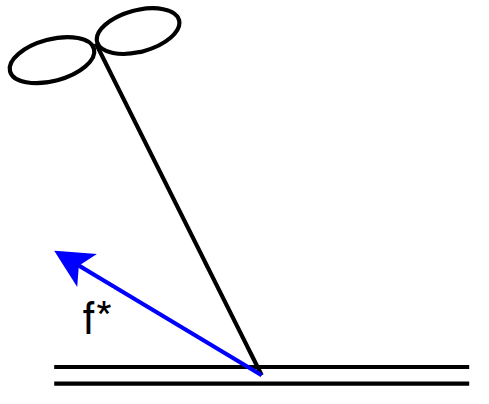
\includegraphics[width=0.3\linewidth]{images/1drone1cableGroundAnchor.png}
    \caption{One drone system connected to the ground through a cable}
    \label{fig:1drone1cableGroundAnchor}
\end{figure}

\subsubsection{Option 1}
Defined the desired cable tension $\tau^*$ and the desired cable direction $u^*$ as:

\begin{minipage}[t]{0.45\textwidth}
  \begin{equation}
    \tau^* = \|f^*\|
    \label{eq:tau_des}
  \end{equation}
\end{minipage}\hfill
\begin{minipage}[t]{0.45\textwidth}
  \begin{equation} 
    u^* = \frac{f^*}{\|f^*\|}
    \label{eq:u_des}
  \end{equation} 
\end{minipage}

\noindent the ground tension is obtained using the geometric constraint which relates the anchor point to the drone position:
\begin{equation}
    a^* = b + l \, u^*
    \label{eq:geometricContraintOnUAV}
\end{equation}
where $l$ is the cable length. Equation \ref{eq:geometricContraintOnUAV} is then used as a reference to compute the propeller force.
\begin{equation}
    F_{prop} =  m_i g e_3 + K_p (a^*-a) + K_d (\dot{a}^* - \dot{a}) + \tau^* u
\end{equation}

\subsubsection{Option 2}
Given the drone Newton's Second Law described in Equation \ref{eq:uavbalance}, we are able to estimate the cable force $\hat{f} = F_{a, i}^{est}$
\begin{equation}
    m_i \ddot{a}_i = F_{prop, i} - \hat{f} + F_{g, i} \qquad \xrightarrow[]{} \qquad \hat{f} = F_{prop, i} + F_{g, i} - m_i \ddot{a}_i
    \label{eq:uavNewton2law}
\end{equation}
where all the forces are in the world frame and $\ddot{a}_i$ is the drone linear acceleration. Using Equation \ref{eq:uavbalance}, we would like to apply a propulsion force equal to 

\begin{equation}    
    F_{prop, i}^* = f^* - F_{g, i}
\end{equation}
Finally, the closed loop equation is:

\begin{equation}
    F_{prop, i} = F_{prop, i}^* + K_p e + K_d \dot{e}
    , \quad \text{with } e = f^* - \hat{f}
\end{equation}
The result is given to the attitude controller, which aligns the body z-axis with the commanded thrust vector.

\subsection{Case: payload connected to the ground and a drone}
In this case, we are working with the simplified case of an ACTS composed by a drone, a ground anchor and a point-mass payload. Called with subscript 1 the cable that connects the payload to the drone and with 2 the one that connects it to the ground, for definition the vector $u_i$, $i = 1\div n$ is given by 
  \begin{equation}
    u_i = \frac{a_i-p}{\|a_i-p\|}
  \end{equation}
being $a_i$ and $p$ respectively the actuator and the payload position.

\subsubsection{Payload position control}
The goal is to design $F_{prop, 1}$ such that the payload reaches a desired position ($p \xrightarrow{}p^*$), which is reachable for the length of the cable.

\begin{figure}[h]
    \centering
    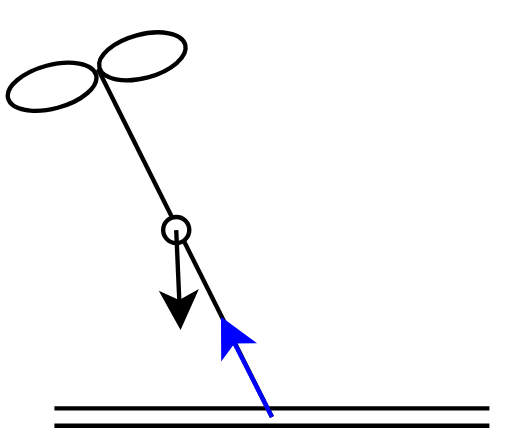
\includegraphics[width=0.3\linewidth]{images/1drone2cablesPayloadGroundAnchorTensionAlongCable.png}
    \caption{Simplified ACTS with one drone and one ground anchor}
    \label{fig:1drone2cablesPayloadGroundAnchorTensionAlongCable}
\end{figure}


The payload dynamics is given by:
\begin{equation}
\begin{aligned}
    m_p \ddot{p} &= \tau_1 u_1 + \tau_2 u_2 - m_p g e_3 \\
    &= F_{a, 1} + F_{a, 2} + F_g \\
    &= F_p + F_g \\
\end{aligned} \quad \xrightarrow[]{}\quad  F_p =m_p (\ddot{p} + ge_3)
\label{eq:Fpdynamics}
\end{equation}
The desired payload force is defined using an impedance controller:
\begin{equation}
    F_p^* = m_p (\ddot{p}^* + ge_3) + K_p (p^*-p) + K_d (\dot{p}^* - \dot{p})
\label{eq:impedancePayloadcontrol}
\end{equation}
with $\dot{p}^*=0$ and $\ddot{p} = 0$ as we required the payload to maintain the position once it is reached. 
The remaining force to be generated by cable 1 is:
\begin{equation}
    F_{a,1}^* = F_p^* - F_{a,2}
\end{equation}
where $F_{a, 2} = \tau_2u_2$. This brings us back to the situation in Section \ref{sec:forceControl1droneToGround}, where $F_{a,1}$ is $f^*$.

\subsubsection{Tension and orientation control}
The goal can also be design $F_{prop,1}$ such that an arbitrary force $f^*$ on the ground can be applied ($F_2 \xrightarrow{} f^*$). In other words, $u_2 \xrightarrow{} u_2^*$ and $\tau_2\xrightarrow{}\tau_2^*$. This case can be interesting to study as in a redundancy system situation, it may be helpful to add additional constraint in one of the cables.
The only difference from the previous case is that the desired position for the payload $p^*$ is not an input anymore, but obtained such that the 2nd cable is aligned along the desired direction given by $f^*$ (Equation \ref{eq:tau_des} and \ref{eq:u_des}). Then:
\begin{equation}
    p^* = a_2 - l_2 u^*_2
\end{equation}

\begin{figure}[h]
    \centering
    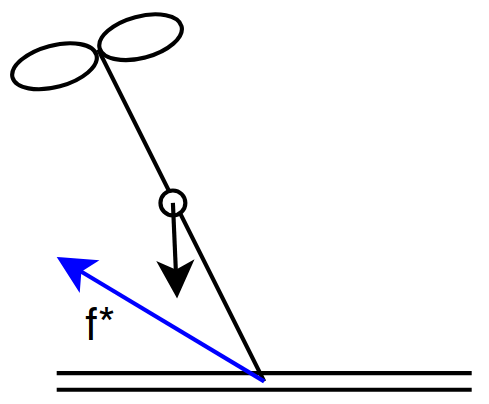
\includegraphics[width=0.25\linewidth]{images/1drone2cablesPayloadGroundAnchor.png}
    \caption{Tension directed arbitrary}
    \label{fig:1drone2cablesPayloadGroundAnchor}
\end{figure}

\subsection{Case: payload connected to the ground through two cables}
The ACTS consists of a point-mass payload connected to the ground through two cables and to an UAV. The enumeration is shown in Figure \ref{fig:1drone2cablesToground}.

\begin{figure}[h]
    \centering
    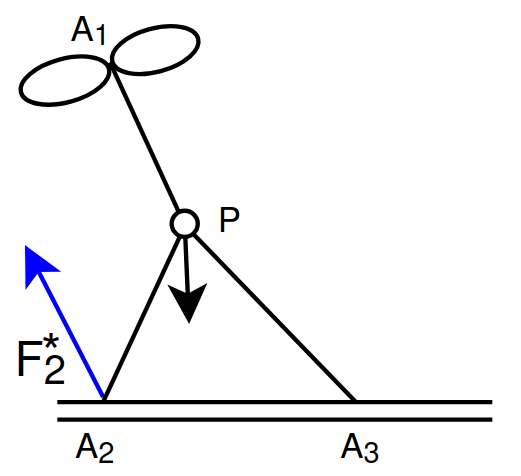
\includegraphics[width=0.3\linewidth]{images/1drone2cablesToground.png}
    \caption{Payload connected through two cable to the ground}
    \label{fig:1drone2cablesToground}
\end{figure}

\subsubsection{Payload position control}
If the input is the desired payload position $p^*$, we find ourselves in three situations:
\begin{enumerate}
    \item $p^*$ lies precisely on the intersecting boundary arcs dictated by the maximum lengths of the ground cables;
    \item $p^*$ is out of reach;
    \item $p^*$ is inside the triangle $A_1A_3P$, resulting into slack cables
\end{enumerate}

In the first case, $p^*$ is used to compute the desired payload force $F_p^*$ (Equation \ref{eq:impedancePayloadcontrol}). Using the simplified payload balance equation related to the forces acting on the payload (Equation \ref{eq:ForceOnPayload}), we obtain the following.
\begin{equation}
    F_{a, 1}^*=F_p^* - \sum_{i=2}^{n} F_{a, i}
\end{equation}
which brings us back to the previous case. 

Because the payload is physically constrained at a boundary where both ground cables are stretched straight, any movement or external disturbance is perfectly resisted by the tension of the cables.

In the second case, since the ground cables physically block the payload from reaching $p^*$, a steady error $e=(p^*-p)\ne 0$ builds up. The actual tension will be directly proportional to the control gains and the distance of the unreachable input:
\begin{equation}
    \sum F_{virtual} \propto (p^* - p_{geom}) \quad \implies \quad \sum F_{virtual} = K (p^* - p_{geom})
\end{equation}
where $p_{geom}$ is the closest reachable point that lies on the workspace boundary. In this case, we may impose a controlled tension on the ground cables directed along $(p^* - p_{geom})$ to ensure the drone continues to pull toward the desired target:

\begin{equation}
    F_{a, 1}^*=F_p^* -\sum_{i=2}^{n} F_{a, i} + F_{virtual}
\end{equation}

In the last case, the distance from the anchors to the payload is less than the cable length, resulting into slack cables as the latter cannot push. Mathematically $\tau_2= 0$ and/or $\tau_3=0$. Then, $F_{a,1}^*= F_p^*$

\subsubsection{Desired tension in the cable on the ground}
The desired variable to control is the tension of one of the cables $F_{a,2} \xrightarrow{} f^*$. 

\begin{equation}
    F_{a, 1}^*=F_p - f^* - F_{a,2}
\end{equation}
where $F_p = m_p (\ddot{p} + ge_3)$ and $F_{a, 2} = \tau_2u_2$.


\subsubsection{Desired tension difference between the cables on the ground}
The desired variable to control a linear combination of the two $F_{a, 2} + \alpha F_{a, 3} \xrightarrow{} f^*$.

\begin{equation}
    F_{a, 1} = F_p - F_{a, 2} - F_{a, 3} 
    \qquad \implies \qquad 
    \begin{aligned}
        F_{a,1}^* &= F_p - (f^* - \alpha F_{a, 3}^* + F_{a, 3}^*) \\
        &= F_p - f^* - (1-\alpha)F_{a, 3}
    \end{aligned}
\end{equation}
For the specific case where $F_{a, 2} - F_{a, 3} \to f^*$:
\begin{equation}
    F_{a,1}^* = F_p - f^* - 2F_{a, 3}^* = F_p - f'^*
\end{equation}
